
\subsubsection{Đường ống dữ liệu Pháp Điển}

Pháp điển là tập hợp các quy phạm pháp luật đang còn hiệu lực của các văn bản quy phạm pháp luật do cơ quan nhà nước ở trung ương ban hành, từ Thông tư trở lên và trừ Hiến pháp.

Sơ đồ tổng quan Data pipeline Pháp Điển


\begin{figure}[H]
\centering
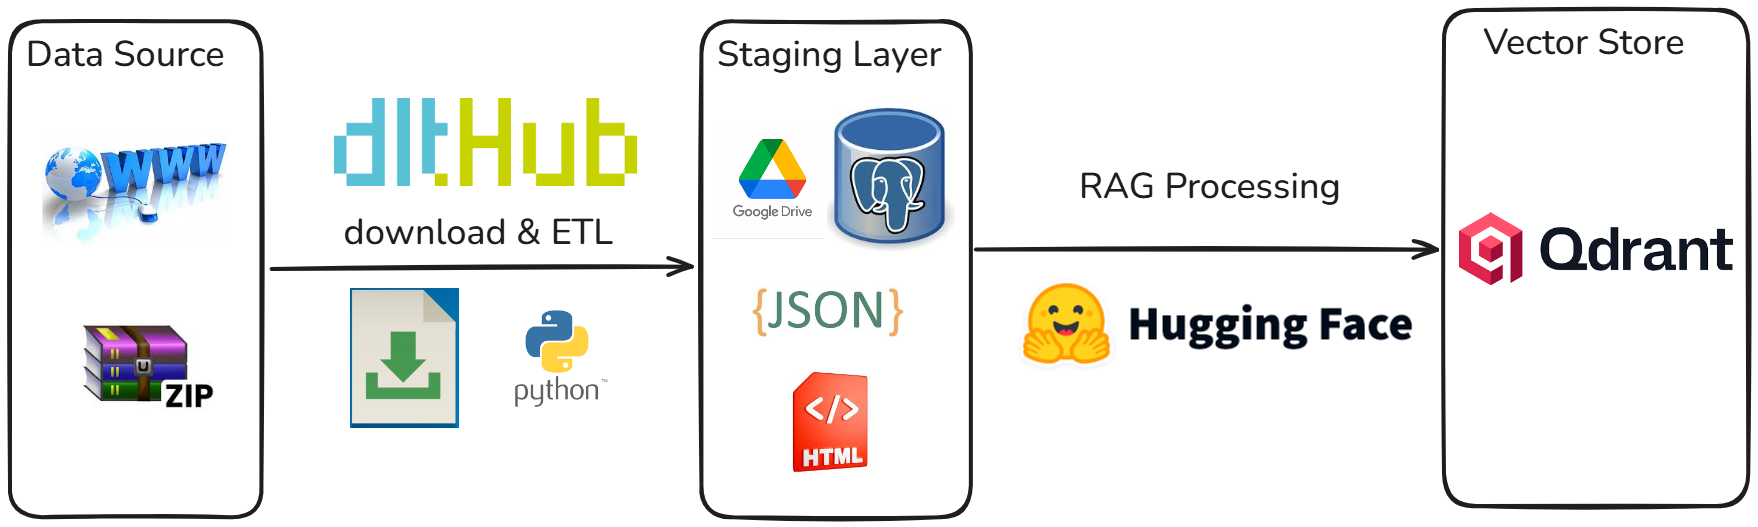
\includegraphics[scale = 0.2]{pictures/Data-Pipeline-PhapDien.excalidraw.png}
\caption{Sơ đồ thu thập dữ liệu chung}
\end{figure}


Tổng quan thông tin file zip


\begin{figure}[H]
\centering
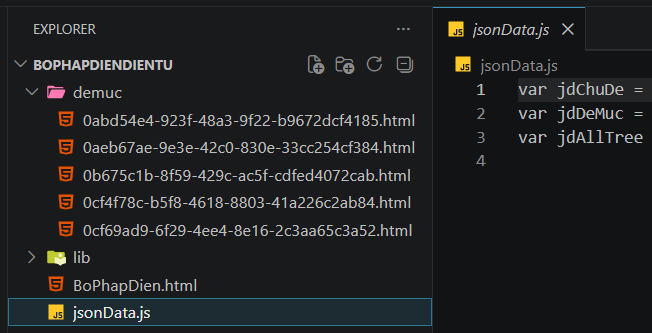
\includegraphics[scale = 0.2]{pictures/zip_file_PhapDien.png}
\caption{Sơ đồ thu thập dữ liệu chung}
\end{figure}


Kết quả file JSON đã trích xuất


\begin{figure}[H]
\centering
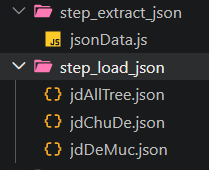
\includegraphics[scale = 0.2]{pictures/step_json_PhapDien.png}
\caption{Sơ đồ thu thập dữ liệu chung}
\end{figure}


Kết quả vector được lưu trong vector database


\begin{figure}[H]
\centering
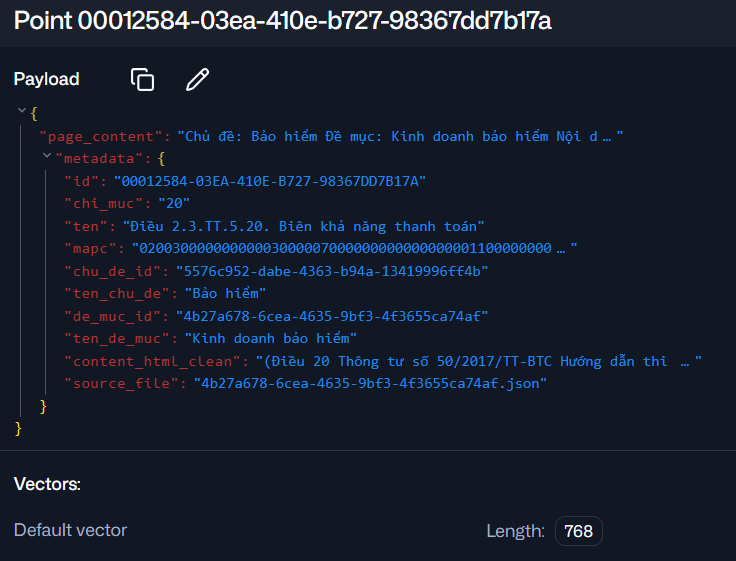
\includegraphics[scale = 0.2]{pictures/vector_database_PhapDien.png}
\caption{Sơ đồ thu thập dữ liệu chung}
\end{figure}


Các bước thực hiện


\begin{figure}[H]
\centering
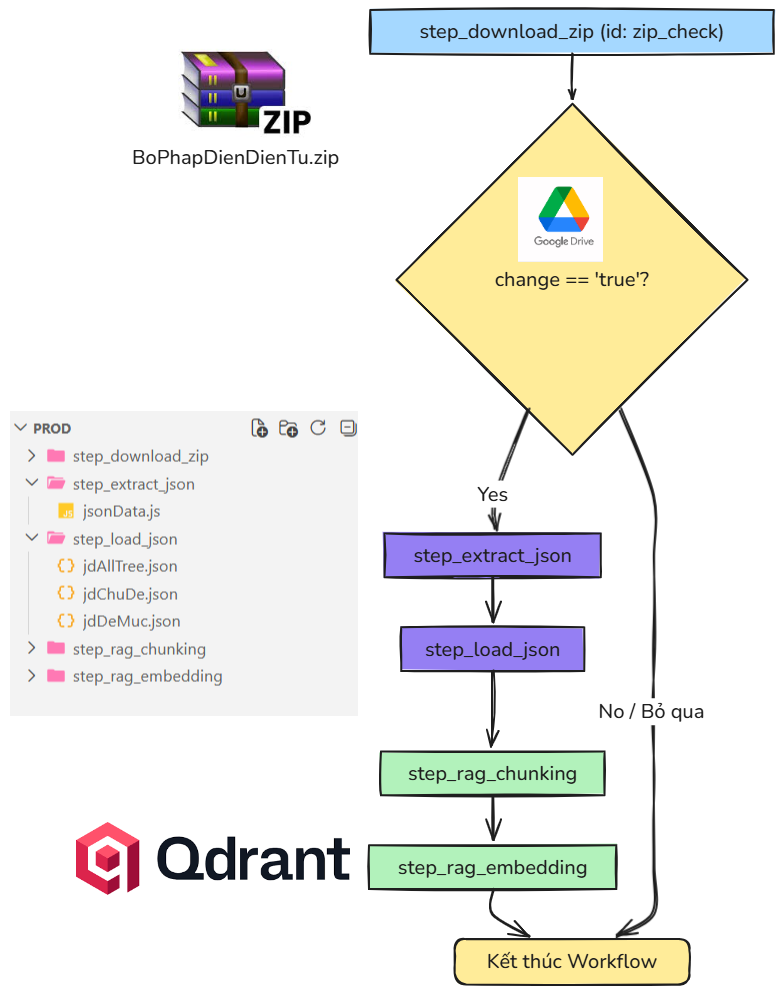
\includegraphics[scale = 0.2]{pictures/step3.excalidraw.png}
\caption{Sơ đồ thu thập dữ liệu chung}
\end{figure}


Mô tả các bước thực hiện:

Quá trình Data pipeline được chia thành 3 giai đoạn: Thu thập dữ liệu, Tiền xử lý văn bản và Tích hợp RAG Pipeline.

- Giai đoạn Thu thập Dữ liệu:

- step\_download\_zip: Tự động tải file nén chứa toàn bộ Bộ pháp điển điện tử ( BoPhapDienDienTu.zip ) từ nguồn Cổng thông tin điện tử pháp điển. Hệ thống tính toán mã băm (MD5) và đồng bộ với Google Drive để kiểm tra sự thay đổi dữ liệu.

- Giai đoạn Tiền xử lý Dữ liệu:

- step\_extract\_json và step\_load\_json: Từ file jsonData.js. Tiến hành bóc tách (parse) các biến cấu trúc dữ liệu để lấy danh sách Chủ đề (jdChuDe), Đề mục (jdDeMuc), và Cây mục lục (jdAllTree), sau đó xuất ra định dạng JSON.

- Giai đoạn Tích hợp RAG Pipeline:

- step\_rag\_chunking: Thực hiện đối chiếu từ Cây mục lục (jdAllTree) với các thẻ bên trong từng file HTML chi tiết. Từ đó, bóc tách chính xác từng phần nội dung văn bản thành dạng JSON có các đoạn văn bản và siêu dữ liệu (Metadata).

- step\_rag\_embedding: Làm giàu ngữ cảnh bằng cách nối trực tiếp tên Chủ đề và Đề mục vào phần đầu của mỗi đoạn văn bản chunk. Sau đó, nội dung được đưa qua mô hình HuggingFace ( keepitreal/vietnamese-sbert ) để biến đổi thành các vector cơ sở dữ liệu vector Qdrant.


\begin{figure}[H]
\centering
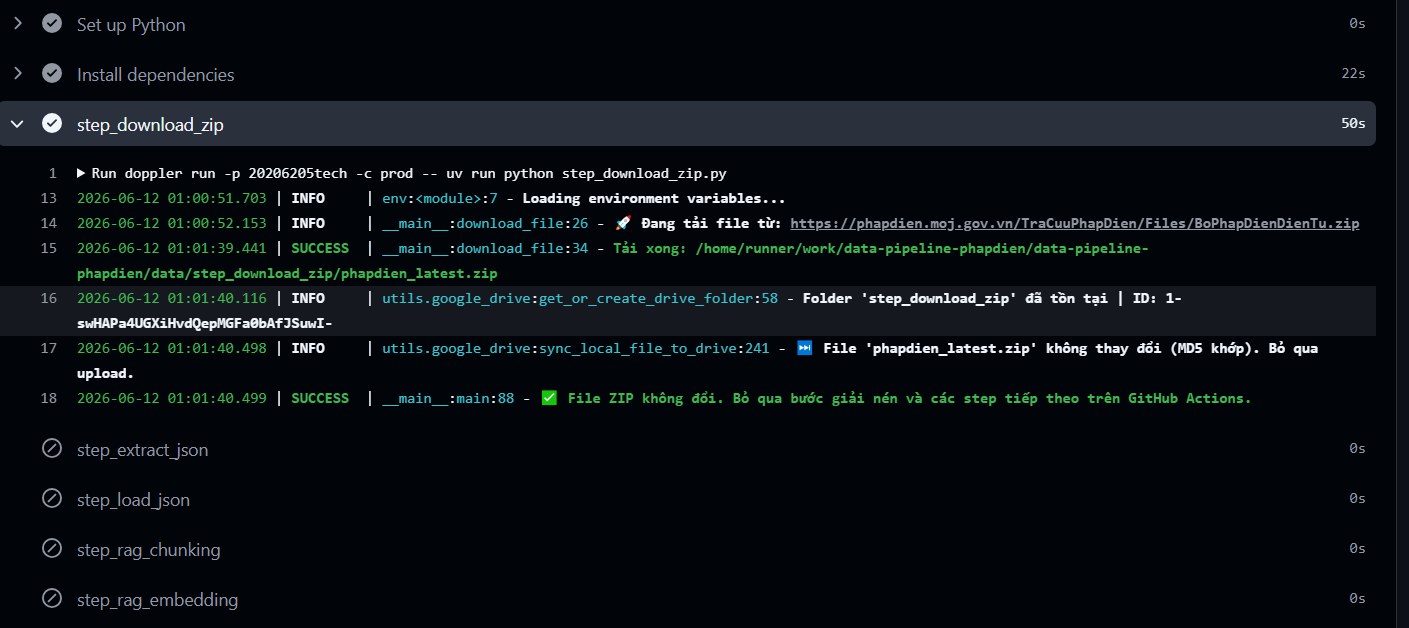
\includegraphics[scale = 0.2]{pictures/github-action-PhapDien.png}
\caption{Sơ đồ thu thập dữ liệu chung}
\end{figure}


\begin{figure}[H]
\centering
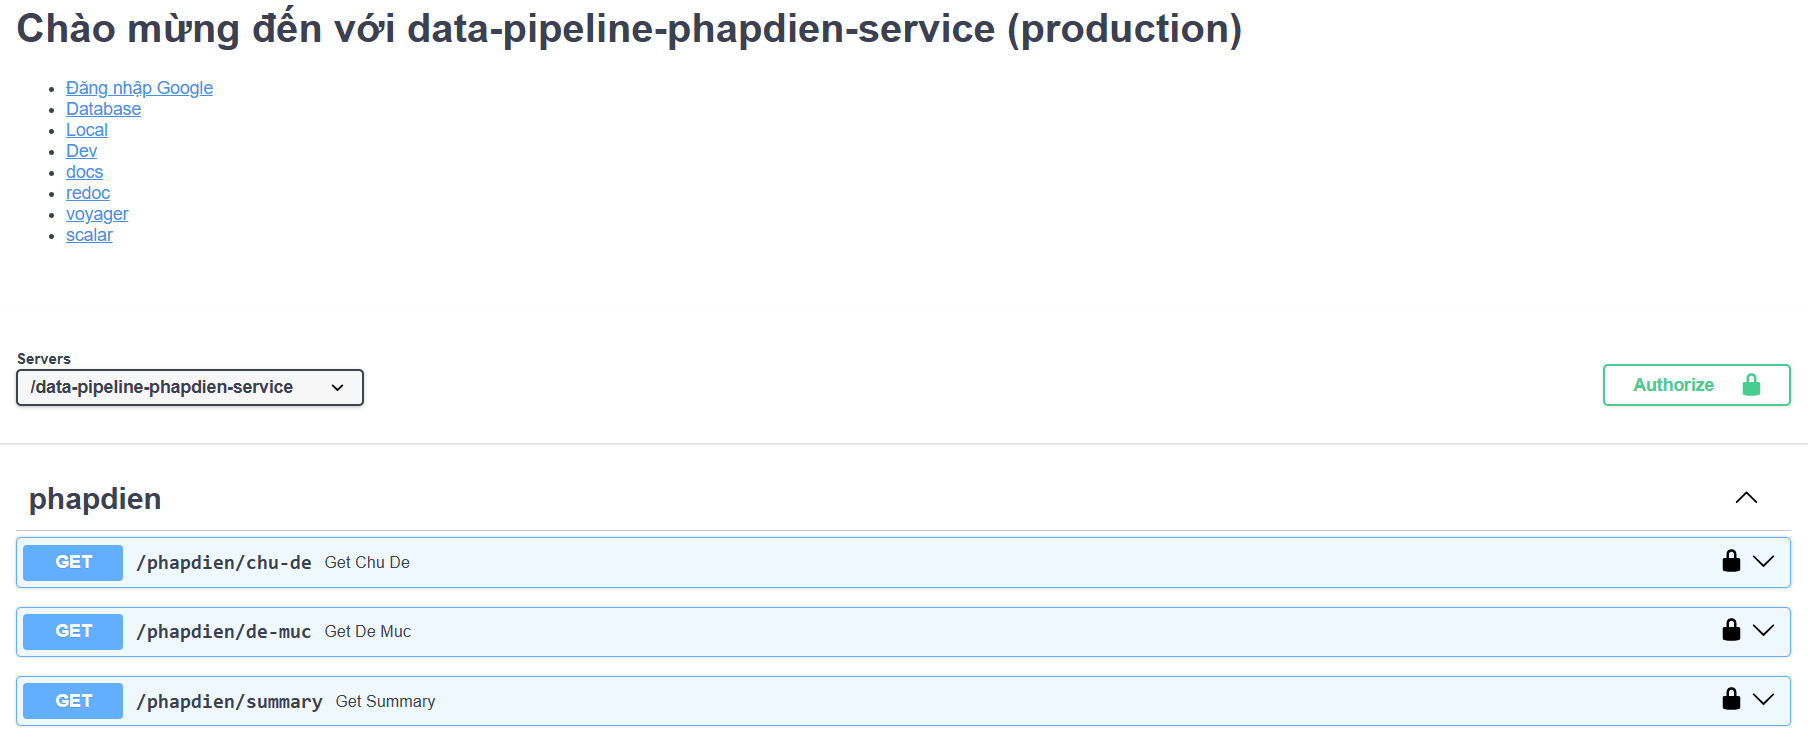
\includegraphics[scale = 0.2]{pictures/PhapDien-SERVICE.png}
\caption{swagger}
\end{figure}

\begin{figure}[H]
\centering
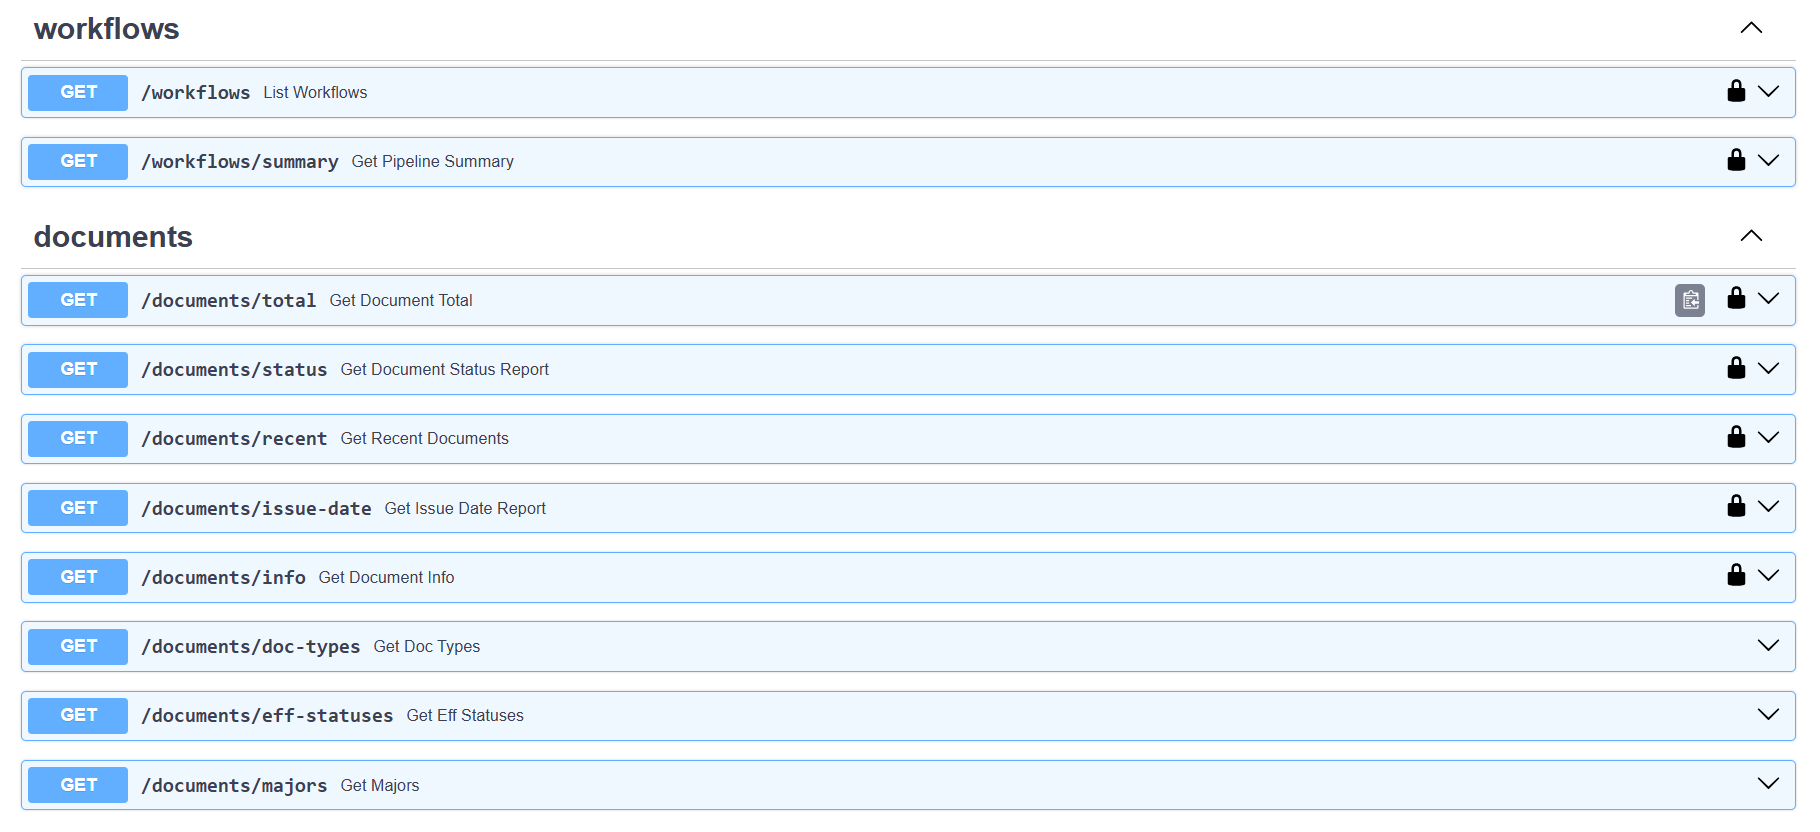
\includegraphics[scale = 0.2]{pictures/VBPL-SERVICE.png}
\caption{swagger}
\end{figure}


\begin{figure}[H]
\centering
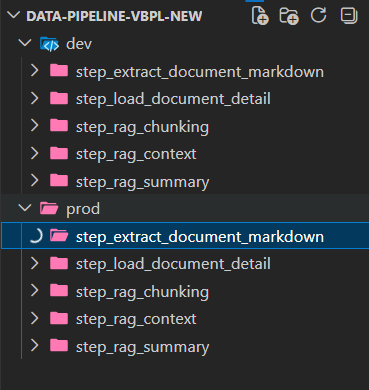
\includegraphics[scale = 0.2]{pictures/google-drive-VBPL.png}
\caption{swagger}
\end{figure}
\begin{figure}[H]
\centering
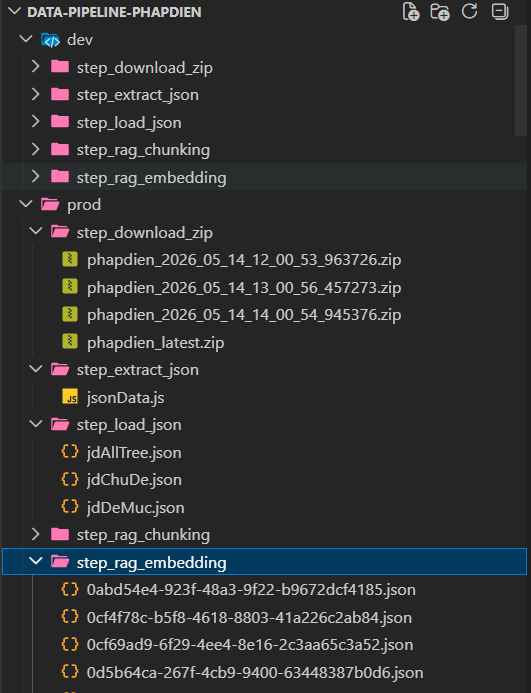
\includegraphics[scale = 0.2]{pictures/google-drive-PhapDien.png}
\caption{swagger}
\end{figure}
